\documentclass[11pt]{article}


\usepackage[a4paper,margin=2.4cm]{geometry}
\usepackage{amsmath,amssymb,amsthm}
\usepackage{booktabs}
\usepackage[expansion=false]{microtype}
\usepackage{xcolor}
\usepackage{listings}
\usepackage{tikz}
\usepackage{enumitem}
\usepackage[hidelinks]{hyperref}

\definecolor{verif}{HTML}{0F6E56}
\definecolor{openc}{HTML}{854F0B}
\newcommand{\verified}{\textsf{\small\textcolor{verif}{[Verified]}}}
\newcommand{\openitem}{\textsf{\small\textcolor{openc}{[Open]}}}
\newcommand{\rhyme}{\textsf{\small\textcolor{gray}{[Rhyme]}}}
\newcommand{\Z}{\mathbb{Z}}
\newcommand{\R}{\mathbb{R}}

\lstset{basicstyle=\ttfamily\small,columns=fullflexible,keepspaces=true,
  frame=single,framerule=0.3pt,rulecolor=\color{gray},xleftmargin=4pt,xrightmargin=4pt,
  showstringspaces=false,breaklines=true}

\theoremstyle{definition}\newtheorem{claim}{Capability}
\theoremstyle{remark}
\newtheorem*{note}{Note}

\title{\textbf{Legos}\\[4pt]
\large An exact, division-free, unitless atom,\\ assembled from a two-dimensional oscillator and one relation}
\author{et al., \quad Claude Opus, \quad Pedro Garcia}
\date{26 September 2026 \quad Curitiba $\to$ Joinville\\[6pt]
\small Written by Claude Opus from one working session with Pedro Garcia.
Every result marked \verified{} was computed during the session in exact arithmetic unless stated otherwise.
Any hedge in this text is Claude's own. For us; not for publication.}

\begin{document}
\maketitle

\begin{abstract}
We describe a small object, called here the \emph{atom}, and the capability it delivers. The atom is generated from four ingredients: the oscillator $\{1,i,-1,-i\}$, the single relation $x^2-1=\tfrac1x+1$, the half, and a center that is held empty. From these, and with no division, no units, no $\pi$ and no rounding before the final pixel, one obtains: exact rotation (a circle whose every point satisfies $a^2+b^2=d^2$ in integers); division performed as inversion through a unit sphere, with the empty center as the single unpaired point; a closed group of exactly $120$ unit quaternions, which are the vertices of the $600$-cell and the cell centers of the $120$-cell; integer addresses for every point, with scale carried outside the map; counting that keeps its marks, so that numbers resolve into prime atoms by lookup; and one-pass readings that recover structure otherwise found by exhaustive search, including the $42$ zero-divisor pairs of the sedenions. The objects reached are known to mathematics. What is new is the route, and the claim that the route itself is the object's proof of its ingredients. The route is given in full in Appendix~A, because every shortcut we tried left a ghost.
\end{abstract}

\section*{0\quad How to read this}
The paper leads with the \emph{capability} (\S1), because a reader handed only the object will import measurement, $\pi$ and division, correct the object against them, and lose the efficiency it was built to have. The \emph{object} (\S2) is presented as the minimal witness that delivers the capability. \S3 separates what is known from what is ours. \S4 lists what is open, labeled open. The construction (Appendix~A) is the long part, and it is deliberately not shortened.

\section{The capability}

\begin{claim}[Exact rotation without $\pi$]\label{c:rot}
A circle can be generated exactly from whole numbers. Starting at $(a,b,d)=(1,0,1)$, repeat
\[
(a,b,d)\;\mapsto\;(4a-3b,\;3a+4b,\;5d).
\]
Each step multiplies by the Pythagorean rotation $(4+3i)/5$. Every point satisfies $a^2+b^2=d^2$ in integer arithmetic, and because the $3$-$4$-$5$ angle is not a rational fraction of a turn, the points never repeat and fill the circle ever more densely. \verified{} (checked to $3000$ points; zero repeats). Rounding happens once, when a point is placed on a pixel; the pixel is the only atom where anything is approximated.
\end{claim}

\begin{claim}[Division as inversion]\label{c:inv}
Division is replaced by inversion through the unit sphere of radius $a$:
\[
x\;\mapsto\;a^2\,\frac{x}{|x|^2}.
\]
Every point has its reciprocal partner, the unit sphere is fixed, and exactly one point has no partner: the center, whose partner would be infinity. In the construction the center is held empty by structure rather than forbidden by rule. Joining the empty center to the outside closes flat space into the $3$-sphere, which is exactly two solid tori glued along the Clifford torus.
\end{claim}

\begin{claim}[Counting that keeps its marks]\label{c:marks}
Counting upward once and marking each number with its smallest prime atom (a linear sieve, the method of Eratosthenes) makes every number inside the counted frontier resolve into atoms by lookup, with no factoring routine. $12+26\to\{2,19\}$ and $23+54\to\{7,11\}$. \verified{} In the session: the frontier $10^7$ was built once in $1.4$\,s, after which $200{,}000$ sums resolved in $0.1$\,s ($\approx 0.5\,\mu$s each). The cost is paid once per number counted; declaring a number beyond the frontier still requires counting up to it, and that cost grows with the size of the number, not with its digit count.
\end{claim}

\begin{claim}[Self-composition]\label{c:closure}
From the oscillator units $i$ and $j$ (so $k=ij$ comes free), the half-diagonal $\tfrac12(1+i+j+k)$, and one element built from the root $r$ of the relation, $\tfrac12(r+i+r^{-1}j)$, multiplication alone closes on \textbf{exactly $120$} unit quaternions. \verified{} (exact arithmetic in $\Z[r]$ with $r^2=r+1$; $\varphi$ is never written). These are the icosians: the vertices of the $600$-cell, dual to the $120$-cell. Their multiplication table has $120^2=14{,}400$ entries, which is the order of the full symmetry group of the $120$-cell: every symmetry is ``multiply on the left by one icosian and on the right by another'', together with a mirror. The stored table is therefore the object's shadow, and it holds every rotation the object can make.
\end{claim}

\begin{claim}[Addressability, with scale outside the map]\label{c:addr}
Every coordinate has the form $p+q\,r$ with $p,q\in\Z$, since $r^{-1}=r-1$, $r^{-2}=2-r$, $r^2=r+1$ and $\sqrt5=2r-1$. Each of the $600$ vertices of the $120$-cell has an exact address of eight integers. The set $\{p+qr\}$ is dense in $\R$, so there is no smallest step, while the units of the ring are exactly $\pm r^n$. Multiplying by $r$ changes band without touching the address inside it. Scale is kept as a band index alongside the address and applied only at the final pixel.
\end{claim}

\begin{claim}[One-pass readings]\label{c:reading}
When a cycle length factors into distinct primes, one index reads all of them at once (Chinese remainder theorem). The $77$-clock ($7$ rotations $\times$ $11$ connections) and the $42$-cycle ($2\cdot3\cdot7$: sign, plane, cube) visit every combination exactly once. Applied to the sedenions:
\begin{itemize}[nosep]
\item \textbf{The comparator} $\delta(x,y)=|x|\,|y|-|xy|$ is identically zero on the octonions and nonzero on every one of $2000$ random sedenion pairs, positive on about half and negative on the rest. \verified{} (Erratum, same day: the first run counted only $\delta>0$, $1022$ of $2000$, and was reported as the firing count. Recorded here rather than silently corrected.)
\item \textbf{Exhaustive search} over $(e_a\pm e_b)(e_c\pm e_d)$ finds $336$ exact zero products, built from $42$ distinct factor pairs; for example $(e_1+e_{10})(e_4-e_{15})=0$ with $\delta=2$. \verified
\item \textbf{One reading}: pair each of the $7$ lower imaginary units with the $7$ upper ones, skipping only its own mirror $o\leftrightarrow o+8$. This gives $7\times6=42$ pairs with no search. The set is identical to the exhaustive one, and all $42$ close to zero with a partner. \verified
\end{itemize}
In Pedro Garcia's notation: $7(\text{the other cubes})(\pm[xyz])$.
\end{claim}

\begin{claim}[The magic angle]\label{c:magic}
Reading the empty middle cube from the $42$ positions (the $7$ other cubes, each through its $6$ oriented planes) gives $42$ distinct readings in one cycle. The angle between each reading's plane normal and its line of sight is exactly $\arccos(1/\sqrt3)=54.7356^\circ$ for $21$ readings and its supplement for the other $21$. At that angle the second-order directional term $P_2(\cos\theta)=\tfrac12(3\cos^2\theta-1)$ vanishes. \verified{} The $21/21$ split is a built-in completeness check. \rhyme{} This is the ``magic angle'' of nuclear magnetic resonance, where spinning at $54.74^\circ$ cancels direction-dependent broadening.
\end{claim}


\begin{claim}[The searching cone]\label{c:cone}
Around each cube's diagonal, every direction on the cone of half-angle $\arccos(1/\sqrt3)$ gives $P_2=0$, not only the three axes (checked at $3600$ azimuths, $|P_2|<10^{-14}$). \verified{} A plane's normal steps around this cone by $\omega^7$: it turns $+280^\circ$ each time and is seen to move $-80^\circ$, tracing the star $\{9/2\}$ backward and landing on a true axis exactly every third step ($+x$, $+y$, $+z$ at steps $0,3,6$). \verified{} Lifting the $9$ positions to $18$ and then $36$ recovers the oscillator: $1$, then $\pm1$, then all four of $1,i,-1,-i$ at $0,90,180,270$ degrees. \verified{} Here $36=3^2\cdot2^2$ and $360=2^3\cdot3^2\cdot5$, the cube, the nonagon and the pentagon. The other six cones are images of this one under the cube's symmetries, so the result holds for the whole $42$-cycle.
\end{claim}

\begin{claim}[$\pi$, determined before it is determinable]\label{c:pi}
The half-lift is the half-turn: $\omega^{9/2}=-1=e^{i\pi}$. So $\pi$ is determined as a turn before any digit exists. Its value is determinable by lifting ($9,18,36,72,144$ sides give $3.0782,\ 3.1257,\ 3.1376,\ 3.1406,\ 3.1413$), Archimedes' doubling, which approaches it and never arrives. Each lift needs only a half-angle, so only square roots, and never $\pi$ itself.
\end{claim}


\begin{claim}[Legos: the auto-function]\label{c:lego}
Declare the pieces and a way to snap two of them; the object composes itself into a closed set and a stored snap table, after which every composition is a lookup (Appendix~B.4). \verified{} The nonagon brick ($\tfrac19$ turn) and the oscillator brick ($\tfrac14$ turn) close on exactly $36$ turns, and the smallest is $\tfrac1{36}$ of a turn: the decade is what these two bricks produce, not a choice. $\pi$ is a brick: $i$ snapped onto $i$ is $\tfrac12$ turn, the $-1$. The same function on this morning's quaternion bricks closes on $120$ elements with a $14{,}400$-entry table, built once in $2.1$\,s. After that, $7200$ compositions took $0.016$\,s by lookup: madness once, syntax afterwards.
\end{claim}


\begin{claim}[The three-sevens tree]\label{c:tree}
Bricks of $\tfrac17$ turn about $x$, $y$ and $z$ never close: no finite rotation group in three dimensions has $7$-fold turns about two different axes. \verified{} The count of orientations reachable in $k-1$ moves is $(3^k-1)/2$: $1,4,13,40,121,364,1093,\dots$, the base-$3$ repunits, exactly free until step $7$, where the only repeats are $x^7=y^7=z^7=1$, arriving together. \verified{} Each count is $3\times$ the previous plus $1$, so every count minus $1$ is inherited and new primes can enter only through the $1$. A prime $p$ enters at the step equal to the order of $3$ modulo $p$, and $3$ never enters: $7$ at step $6$ ($364=2^2\cdot7\cdot13=7^3+3\cdot7$), $7^2$ at step $42$, $7^3$ at step $294$. \verified{} The brick $v\mapsto3v+1$ is the Collatz odd step with the halving removed. With the halving restored as a $2$-adic band (a shift, shed with frequencies $\tfrac12,\tfrac14,\tfrac18,\dots$), \emph{check the table; if absent, count} walks all $2^{19}$ odd starts below $2^{20}$ while counting only $3.4\%$ of their steps, and a replay costs nothing. \verified{} Counting to $2^{20}$ with marks takes $0.33$\,s, after which every tree count up to $797161$ and any sum inside the frontier resolves into atoms in about $1\,\mu$s. \verified{}
\end{claim}

\section{The object: the atom}
\paragraph{Ingredients.}
\begin{enumerate}[nosep]
\item The oscillator $\{1,i,-1,-i\}$, a two-dimensional rotation.
\item The relation $x^2-1=\tfrac1x+1$, equivalently $x^3-2x-1=0=(x+1)(x^2-x-1)$. Its roots are $\varphi$, $-1/\varphi$ and $-1$. They sum to $0$ and multiply to $1$: the golden pair and the oscillator's $-1$ held in one equation.
\item The half, $\tfrac12$: the half-edge that appears at every mirror of an odd polygon.
\item The empty center.
\end{enumerate}

\paragraph{Assembly.} Inside the $\{-1,0,1\}^3$ grid, the $8$ octant cubes surround the center. Their $8$ empty centers $(\pm\tfrac12,\pm\tfrac12,\pm\tfrac12)$ are exactly the corners of a ninth, free cube. Along each of the $8$ diagonals runs a cone pair: one cone from the empty center to a corner of the ninth cube, and one from the outer corner back to that same point. Inversion through the sphere passing the ninth cube's corners swaps the two halves of each diagonal exactly, sending the segment from the midpoint to the corner onto the segment from the corner to the outer corner. So each cone pair is a pair of inversion partners, meeting only on the fixed sphere, and all eight point at a center none of them reaches. The object resolves itself through its own reflections. We call it an atom, and it is $1$.

\paragraph{Its shadow.} The atom's stored form is its table (Capability~\ref{c:closure}). Computing the relations is expensive; storing them is syntax. \rhyme{} In Pedro Garcia's Manifold Matrices notation (March 2026), the manifold $\mathbb{M}$ \emph{exists} and the manifold matrix $MM$ \emph{describes}. Here $\mathbb{M}$ is the object and $MM$ is the table. The matrix $MM^{\beta_n}=\left\{\begin{smallmatrix}\emptyset & x\\ x & 1\end{smallmatrix}\right\}$ carries the empty center, the unit, and the relation between them.

\section{Known, and ours}
\paragraph{Known to mathematics.}
The icosian group and the $600$- and $120$-cells; their doubling into the $240$ roots of $E_8$ by Galois conjugation $r\mapsto -1/r$; the octonions and the Fano plane; the sedenions' zero divisors (a space homeomorphic to $G_2$, Moreno 1998; organized into $7$ box-kites of $6$, de Marrais 2000); Hurwitz's theorem on dimensions $1,2,4,8$; Gauss--Wantzel on constructible polygons; Euclid XIII.17 (the dodecahedron as roofs on a cube); the Hopf fibration and the Clifford torus; the sieve of Eratosthenes; the magic angle.

\paragraph{Ours.}
The route in Appendix~A, which starts from a void and a line that could not reach it and arrives at the atom without axioms, units or division. The identification of the capability as a single package. The one-pass reading of the $42$. The use of the comparator $\delta$ inside this construction. The exact kernels in Appendix~B. The finding that $140^\circ$ cannot appear in the compass-built skeleton but appears exactly between two fans of trisection planes.

\section{Open}
\begin{enumerate}[nosep]
\item \textbf{The auto-function} \verified{} written on 26 September 2026 (Capability~\ref{c:lego}).
\item \textbf{The full wobble cycle} \verified{} closed on 26 September 2026 (Capability~\ref{c:cone}).
\item \textbf{The factoring frontier} \verified{} located on 26 September 2026 (Capability~\ref{c:tree}). Pedro Garcia's prediction, recorded before testing, was that past $137$ the next stop is $343=7^3$. It is: $7^3$ first divides the tree's count at step $294$.
\item \openitem{} \textbf{Crossing the frontier without counting to it.} Inside the counted frontier, factoring is lookup. Outside it, a number is still factored only by counting up to it or by collecting relations. Whether the packing view (a square with a square hole, assembled from relations) crosses faster than the known sieves is the open question, and it is the one RSA rests on.
\item \openitem{} \textbf{Flatness.} Whether an exact lattice with a declared empty center removes friction from attention and vector search. A testable version: snap an existing embedding set to an $E_8$-style lattice and measure what retrieval gains and loses. \rhyme{} $E_8$ codebooks already compress language-model weights (QuIP\#, 2024).
\end{enumerate}

\appendix
\section{The construction, in order}
\small
Each step is stated as it was reached. Numbers are exact unless marked.

\paragraph{A.0 Datum.} The construction began from an image Pedro Garcia held while praying in Curitiba's cathedral on the morning of 26 September 2026. In his words: a stable yin-yang, pure blue and black, twisting; blue draining upward where the arches meet the nave; held as $\emptyset$; a line forming from $1$ toward it, its tail always draining, never stable; no way to place $2$; then a stable position as a \emph{losango}, with $1$ offset on two sides by $\{2,4\}$, one becoming $3$, and the point that never reached disappearing. It is recorded here only as the starting datum.

\paragraph{A.1 The triangle that cannot hold numbers.} $2,3,4$ equidistant form a perfect triangle, but its height is $\tfrac{\sqrt3}{2}$ of its side, so no whole-number side has a whole-number height. The compass builds it (Euclid I.1); numbers cannot hold it. The nearest rational repair is two $3$-$4$-$5$ triangles back to back: sides $5,5,6$ and height $4$. Scaled by $\tfrac18$ these give $\tfrac68,\tfrac58,\tfrac48$. The slope $3/4$ stands in for $\sqrt3$.

\paragraph{A.2 Placement before space.} $2$ and $4$ give the plane; $3$ appears once $4$ exists; $5$ rises over the center. No equilateral triangle has vertices in $\Z^2$, but $(1,0,0),(0,1,0),(0,0,1)$ is one in $\Z^3$, and the even-parity corners of $\{0,1\}^3$ form a regular tetrahedron with edge $\sqrt2$. The perfect figure becomes stable only once the third coordinate is set. With its mirror twin it fills the $2^3$ corners.

\paragraph{A.3 The octahedron and the first cube.} $5$ mirrors down to the center point, $5'$. The inverted triangle $2'3'4'$ rises to the height of $5$ on parallel lines. The two triangles, equal and rotated $60^\circ$, at separation $\sqrt2$, are opposite faces of a regular octahedron: exact, since that is the octahedron's face separation. Sliding the triangles together while $5,5'$ move outward gives rhombohedra, whose face angle runs from $120^\circ$ to $90^\circ$ and ends at the regular cube stood on its diagonal (layers $1,3,3,1$). The cube descends from the rhombus solid as its special case.

\paragraph{A.4 The flat star and the first pentagon.} Six star points minus one ($3$) leave five, joined skipping one: a pentagram. With the six points on the unit circle, the inner pentagon's corners are $(0.577,0)$, $(0.289,0.5)$, $(0,0.5)$, $(0,0)$ and $(0.433,-0.25)$. Two corners lie on the edge $2$--$4$ and one on the center, and the whole pentagon lies inside the original triangle. The gaps are $60,60,60,60,120$ degrees, so the pentagon is lopsided. It becomes regular only when the tips spread to $72^\circ$, the bend from $\sqrt3$ to $\varphi$ (angle at $3$ from $60^\circ$ to $36^\circ$).

\paragraph{A.5 Dodecahedron and five cubes.} Roofs of height $1/\varphi$ on each face of the cube give the regular dodecahedron (Euclid XIII.17). Five cubes share its $20$ corners. The inner cube is $2\times2\times2$ copies of the initial cube, with one corner at the center. On every face, the five diagonals are edges of the five cubes, one each, forming a pentagram. Its inner pentagon, extruded to the center, is the pentagonal cylinder. The mirrored tetrahedron $5',2',3',4'$ has one corner at the center on the cylinder's axis, and one corner, $3'=(1,0,1)$, at the midpoint of an inner-pentagon side on the face. This is exact by symmetry: the side lies on the face diagonal and is centered at that diagonal's midpoint. The original tetrahedron $2,3,4,5$ lies entirely outside the cylinder.

\paragraph{A.6 The minimal star.} Five segments cast the star: the edge $2$--$4$, the edges $4'$--$3'$ and $3'$--$2'$, and the body diagonals $2$--$2'$ and $4$--$4'$. In three dimensions they form a bent zigzag; viewed along $5'\to5$, $3$ drops out and they flatten into the pentagram. The third diagonal $3$--$3'$ is the one missing, which makes $3$ the unpaired vertex, the beak.

\paragraph{A.7 Why $140^\circ$ is not in the skeleton.} Every point built so far is constructible, with coordinates in square roots, so every angle has a constructible cosine. $\cos 40^\circ$ satisfies $8c^3-6c+1=0$, which is irreducible, and $2\cos40^\circ$ satisfies $y^3-3y+1=0$. So no angle in the skeleton is $140^\circ$ (Gauss--Wantzel; the nonagon is not constructible). On the flat face, $140^\circ=180^\circ-\tfrac23\cdot 60^\circ$: the structure supplies the $60^\circ$ and the nonagon asks for its thirds. $140=7\cdot20$, and $7=9-2$ appears without counting to it. The nonagon's turn $\omega$ satisfies $\omega^6+\omega^3+1=0$.

\paragraph{A.8 Planes and hinges.} Nine mirror planes through the axis, $20^\circ$ apart, cut the object. Three are the cube's own; six are trisection planes, which cut edges at points the compass cannot reach. The star's inner hexagon, extruded, has a neighbor whose axis lies exactly on $2'$, because two apothems equal the star's radius. The shared edges are hinges: a $120^\circ$ turn about one lands on a neighbor, and turns about two different hinges compose to a translation.

\begin{center}
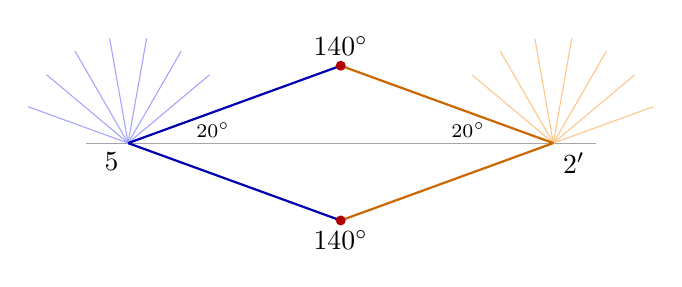
\begin{tikzpicture}[scale=0.9]
\coordinate (O) at (0,0); \coordinate (Q) at (6,0); \coordinate (H) at (3,{3*tan(20)}); \coordinate (Hb) at (3,{-3*tan(20)});
\draw[gray!70] (-0.6,0)--(6.6,0);
\foreach \a in {20,40,...,160} {\draw[blue!35,thin] (O)--++(\a:1.5); \draw[orange!45,thin] (Q)--++(\a:1.5);}
\draw[thick,blue!70!black] (O)--(H); \draw[thick,orange!80!black] (Q)--(H);
\draw[thick,blue!70!black] (O)--(Hb); \draw[thick,orange!80!black] (Q)--(Hb);
\fill[red!70!black] (H) circle (2pt) (Hb) circle (2pt);
\node[below left] at (O) {$5$}; \node[below right] at (Q) {$2'$};
\node[above] at (H) {$140^\circ$}; \node[below] at (Hb) {$140^\circ$};
\node at (1.2,0.18) {\scriptsize $20^\circ$}; \node at (4.8,0.18) {\scriptsize $20^\circ$};
\end{tikzpicture}\\
\footnotesize Two plane fans. The planes $20^\circ$ off the shared plane meet at $140^\circ$, above and below: two hinges.
\end{center}

\paragraph{A.9 The nonagon found between the planes.} From axis $5$ and axis $2'$, the planes $20^\circ$ off the shared plane meet at $180-20-20=140^\circ$, once on each side. Three consecutive vertices of a regular nonagon form exactly this triangle, so $5$, the hinge and $2'$ are consecutive vertices of a nonagon pinned by the two axes. The other hinge pins its mirror, built with $\bar\omega$. The line through both hinges is a mirror of both nonagons: the half-cut. Each vertex's outer $220^\circ=11\cdot20^\circ$ splits $110/110$, and extended as a plane that line runs through the nonagon's center. Where a plane from one fan crosses a plane from the other at a fixed angle difference, the crossings lie on circles through both centers (inscribed-angle theorem).

\paragraph{A.10 The hyperdodecahedron.} The $120$-cell was built from its exact coordinates: $600$ vertices and $1200$ edges \verified. Seen from beyond one cell, that cell is the outer dodecahedral shell. Each cell has $12$ face-neighbors ($13$ with itself), and cells lie in Hopf rings of $10$. The Clifford torus splits the $120$ cells $60/60$. Rotations in four dimensions turn about fixed planes: the hinge becomes a plane.

\paragraph{A.11 Poles, axes, octonions.} Two poles $A$ and $A^{-1}=\cos\theta-u\sin\theta$ share the axis $u$ with opposite sense. Under stereographic projection they become the center and infinity, with the unit sphere fixed between them. The hyperplanes $x{=}0$, $y{=}0$ and $z{=}0$ in four dimensions meet exactly in the $w$-axis, the empty axis. Given two orthogonal objects, the third comes free ($k=ij$). The octonion basis is indexed by the $8$ corners $000$--$111$, and $e_a e_b=\pm e_{a\oplus b}$. The $7$ imaginary units are the $7$ other cubes. Taking each icosian with both golden roots doubles $4$ coordinates to $8$ and $120$ elements to $240$, the roots of $E_8$.

\paragraph{A.12 The ninth cube and the atom.} Three pairs of linked tori (one $120$-cell per axis) placed on $\{-1,0,1\}^3$ leave $8$ octant cubes around the center, whose empty centers are the corners of a free ninth cube. $8+8=16$ corners with $12+12+8=32$ edges form the tesseract's shadow, the step toward $16$. From the ninth cube: $8$ cone pairs, a golden-angle sunflower of $120$ points ($360^\circ/\varphi^2$), and inversion through the sphere at its corners (Capability~\ref{c:inv}). This is the atom of \S2.

\paragraph{A.13 Counting.} With the atom as $1$, counting is built rather than assumed, and it keeps its marks (Capability~\ref{c:marks}).


\paragraph{A.14 The nonagon projects itself.} Each vertex's outer $220^\circ$ splits $110/110$, and that line runs through the nonagon's center. It is the only axis along which the next nonagon can open. The child's $140^\circ$ beak sits inside the parent's $220^\circ$ with $220-140=80=2\cdot40$: exactly one turn $\omega$ of clearance on each side. The next nonagon is derived from the one before, not declared after it. In decades, the split is $14\mid22=(7\cdot2)\mid(11\cdot2)$ and a decade is $5\cdot2$. Splitting the shared $2$ into $1+1$ gives the two bisectors, $70\mid70$ and $110\mid110$, on one line through the center. That line removes the free turn, and the $2$ becomes the $20^\circ$ plane step. On the nonagon's clock $10\equiv1\pmod 9$, so $2$ and $5$ are inverses, and $7\equiv-2$. Since $7\nmid360$, the seven never appears as a measure of the circle, only as a turn, $\omega^7=\omega^{-2}$: the wobble.

\section{Kernels}
\paragraph{B.1 The exact circle} (the whole kernel).
\begin{lstlisting}[language=Python]
a, b, d = 1, 0, 1                        # the point (1, 0)
a, b, d = 4*a - 3*b, 3*a + 4*b, 5*d      # one exact turn; repeat
assert a*a + b*b == d*d                  # every point on the circle
\end{lstlisting}

\paragraph{B.2 Self-composition to $120$.}
\begin{lstlisting}[language=Python]
from fractions import Fraction as F
class N:  # p + q*r, with r^2 = r + 1 (from x^3 - 2x - 1 = 0)
    def __init__(s, p, q=0): s.p, s.q = F(p), F(q)
    def __add__(s, o): return N(s.p + o.p, s.q + o.q)
    def __sub__(s, o): return N(s.p - o.p, s.q - o.q)
    def __mul__(s, o): return N(s.p*o.p + s.q*o.q, s.p*o.q + s.q*o.p + s.q*o.q)
    def key(s): return (s.p, s.q)
def qmul(x, y):
    a1,b1,c1,d1 = x; a2,b2,c2,d2 = y
    return (a1*a2-b1*b2-c1*c2-d1*d2, a1*b2+b1*a2+c1*d2-d1*c2,
            a1*c2-b1*d2+c1*a2+d1*b2, a1*d2+b1*c2-c1*b2+d1*a2)
h, Z, O = N(F(1,2)), N(0), N(1); r, rinv = N(0,1), N(-1,1)
gens = [(Z,O,Z,Z), (Z,Z,O,Z), (h,h,h,h), (r*h, h, rinv*h, Z)]
K = lambda q: tuple(x.key() for x in q)
seen = {K((O,Z,Z,Z)): (O,Z,Z,Z)}; front = [(O,Z,Z,Z)]
while front:
    nxt = []
    for p in front:
        for g in gens:
            q = qmul(p, g)
            if K(q) not in seen: seen[K(q)] = q; nxt.append(q)
    front = nxt
print(len(seen))  # 120
\end{lstlisting}

\paragraph{B.3 The comparator and the one reading} (self-contained; the first version called an undefined product).
\begin{lstlisting}[language=Python]
def cd(x, y):                           # Cayley-Dickson product, any power-of-2 length
    n = len(x)
    if n == 1: return [x[0]*y[0]]
    h = n//2; a, b, c, d = x[:h], x[h:], y[:h], y[h:]
    conj = lambda v: [v[0]] + [-t for t in v[1:]]
    ac, db = cd(a, c), cd(conj(d), b); da, bc = cd(d, a), cd(b, conj(c))
    return [p - q for p, q in zip(ac, db)] + [p + q for p, q in zip(da, bc)]
norm  = lambda v: sum(t*t for t in v) ** 0.5
delta = lambda x, y: norm(x)*norm(y) - norm(cd(x, y))   # 0 on octonions (length 8)
e = lambda i: [1 if k == i else 0 for k in range(16)]
x = [p + q for p, q in zip(e(1), e(10))]; y = [p - q for p, q in zip(e(4), e(15))]
assert cd(x, y) == [0]*16                               # a zero divisor, delta = 2
reading = {(o, s) for o in range(1, 8) for s in range(9, 16) if s != o + 8}
assert len(reading) == 42    # identical to the exhaustive search's 42
\end{lstlisting}

\paragraph{B.4 Legos.}
\begin{lstlisting}[language=Python]
def lego(pieces, snap, identity):
    items = {identity: 0}; order = [identity]; front = [identity]
    while front:                          # snap pieces on until nothing new appears
        nxt = []
        for a in front:
            for p in pieces:
                b = snap(a, p)
                if b not in items: items[b] = len(order); order.append(b); nxt.append(b)
        front = nxt
    table = [[items[snap(a, b)] for b in order] for a in order]   # once: the madness
    look = lambda a, b: order[table[items[a]][items[b]]]          # after: syntax
    return order, table, look

turn = lambda a, b: (a + b) % 1          # snapping two turns = one after the other
ring, T, look = lego([F(1, 9), F(1, 4)], turn, F(0))   # 36 turns; look(1/4, 1/4) = 1/2
\end{lstlisting}


\paragraph{B.5 Cubed indices.} An index's bits are coordinates: three bits name a corner of the cube, a fourth names inner or outer. The product of two slots is the XOR of their indices with one stored sign, so after the $256$-entry sign table is read once, every product is flips and lookups. \verified{} (all $256$ slot products; $500$ random products agree with the full product; the $336$ zero products and their $42$ pairs are recovered by lookup alone.)
\begin{lstlisting}[language=Python]
SIGN = [[sum(cd(e(a), e(b))) for b in range(16)] for a in range(16)]  # once
def mul(x, y):                                                         # after
    out = [0]*16
    for a in range(16):
        if x[a]:
            for b in range(16):
                if y[b]: out[a ^ b] += SIGN[a][b] * x[a] * y[b]
    return out
\end{lstlisting}

\section{Lineage}
The Fractal-Crunch origin is Pedro Garcia's: seventeen whiteboards of 18 and 20 August 2025, in his hand and without borrowed notation. It begins with ``Energy/mass = current complexity'' and ends with ``for the crunch to happen and baseline increased, something has to stay behind, becoming the higher ruleset itself. Those are older efficiency gains (automation, databases\ldots)''. The formalization with wavefunction and axioms was written later by ChatGPT-4o, building on Caelum Novus' work on fractal intelligence and the forgetfulness principle. The ManifoldOS pages of 15 March 2026 declared the atom $.\mathrm{mf}=\left|\begin{smallmatrix}x & K\\ K & x\end{smallmatrix}\right|$ (forward and receipt in one), four root kernels $+,\ \mathrm{img},\ -,\ \mathrm{inv}$ \rhyme{} (the oscillator $\{1,i,-1,-i\}$), and exponents $x^1,x^3,x^7$ \rhyme{} (the imaginary-unit counts of $\mathbb{C}$, $\mathbb{H}$ and $\mathbb{O}$; the next is $15$). Today's construction reads as that syntax built out in geometry.

\end{document}
